\section{Решение}

\subsection{Модель 1}

Трёхслойная осесимметричная модель:

\begin{table}[h]
\centering
{\setlength\tabcolsep{2pt}
\begin{tabular}{r c l} %\setlength\intextsep{0mm}
    первый слой &---& скважина (${0 < r < 1}$) с УЭС ${\rho_\text с = 1}$, \\
    второй слой &---& зона проникновения (${1 < r < r_\text{зп} = 4}$) с УЭС ${\rho_\text{зп} = 4}$, \\
    третий слой &---& пласт (${r > r_\text{зп}}$) с УЭС $\rho_\text{п}$.
\end{tabular}}
\end{table}

На рис. \ref{fig:curves_1} решение потенциального поля, кажущихся сопротивлений потециал- и градиент-зондов в скважине. Решение потенциального поля на рис. \ref{fig:field_1_1} и \ref{fig:field_1_2}.

На рис. \ref{fig:field_1_2} наблюдаются разрывы градиента потенциального поля на границах зон и сингулярность поля в точке источника потенциала, означает, что это не классичекое решение задачи, а более общее --- обобщенное решение задачи. 

Время вычисления решения ${1.24 \text{ c } \pm 38.3 \text{ мс}}$, 7 проходов
(среднее значение${\ \pm \ }$среднеквадратичное отклонение от 7 проходов, в каждом проходе 1 цикл) c 6409 узлами расчетной сетки на рис. \ref{fig:mesh_1_1} и \ref{fig:mesh_1_2}.

Решение палетки на рис. \ref{fig:palette_1} с расчетной сеткой на рис. \ref{fig:mesh_1_1}.

На рис. \ref{fig:palette_1} наблюдаются вырождение кривых в одну кривую при меньших длин зонда и асимптотическое поведение кривых при меньших длин зонда и при больших длин зонда. Асимптота при меньших длин зонда есть горизонтальная прямая со значением УЭС скважины $\rho_\text{с}$. Асимптота при больших длин зонда есть горизонтальная прямая со значением УЭС пласта $\rho_\text{п}$.

Время вычисления расчетной палетки ${18 \text{ c } \pm 159 \text{ мс }}$, 7 проходов.

Сравнены расчетная и известная палетки на рис. \ref{fig:compare_1}. Наблюдается совпадение, означает, что способ решения верный и точный.

\begin{figure}[H]
\centering
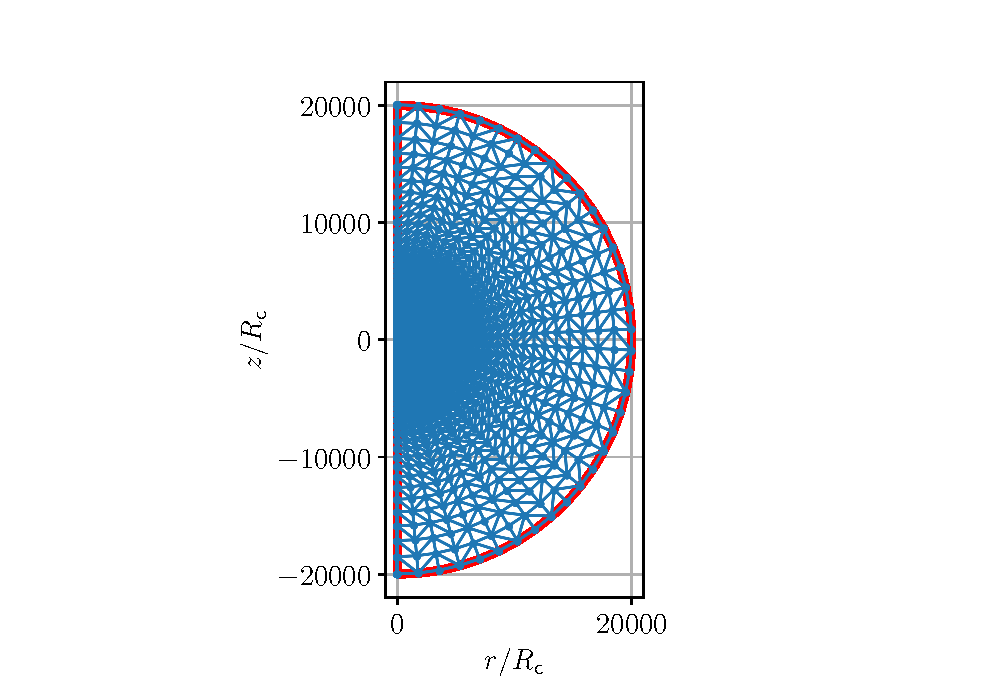
\includegraphics{plot_1_tg_1}
\caption{Триангуляция}
\label{fig:mesh_1_1}
\end{figure}

\begin{figure}[H]
\centering
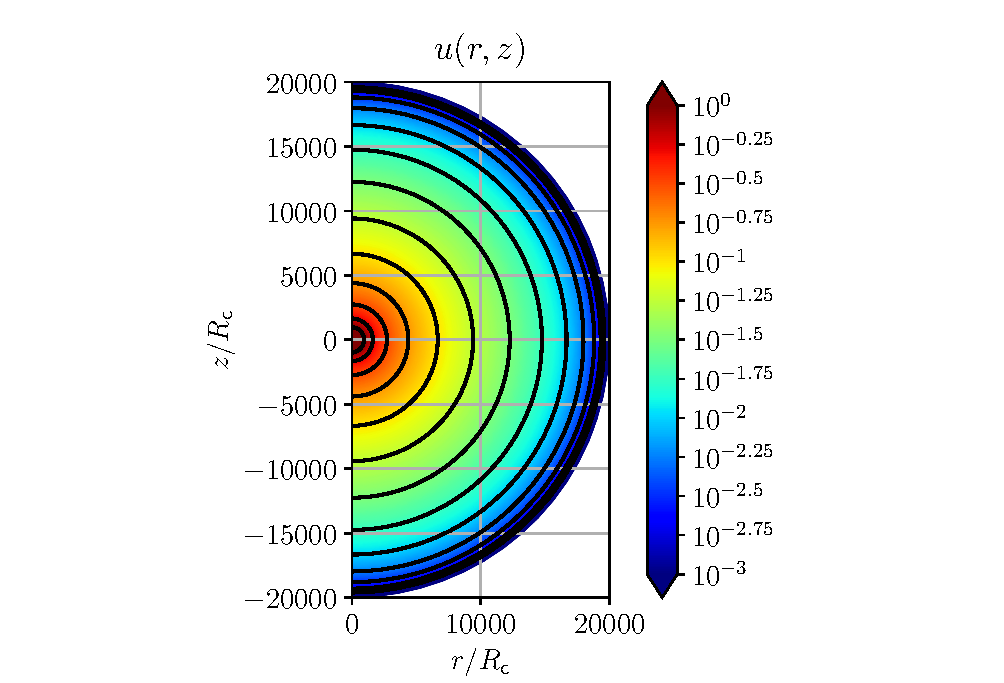
\includegraphics{plot_1_field_1}
\caption{Потенциальное поле}
\label{fig:field_1_1}
\end{figure}

\begin{figure}[H]
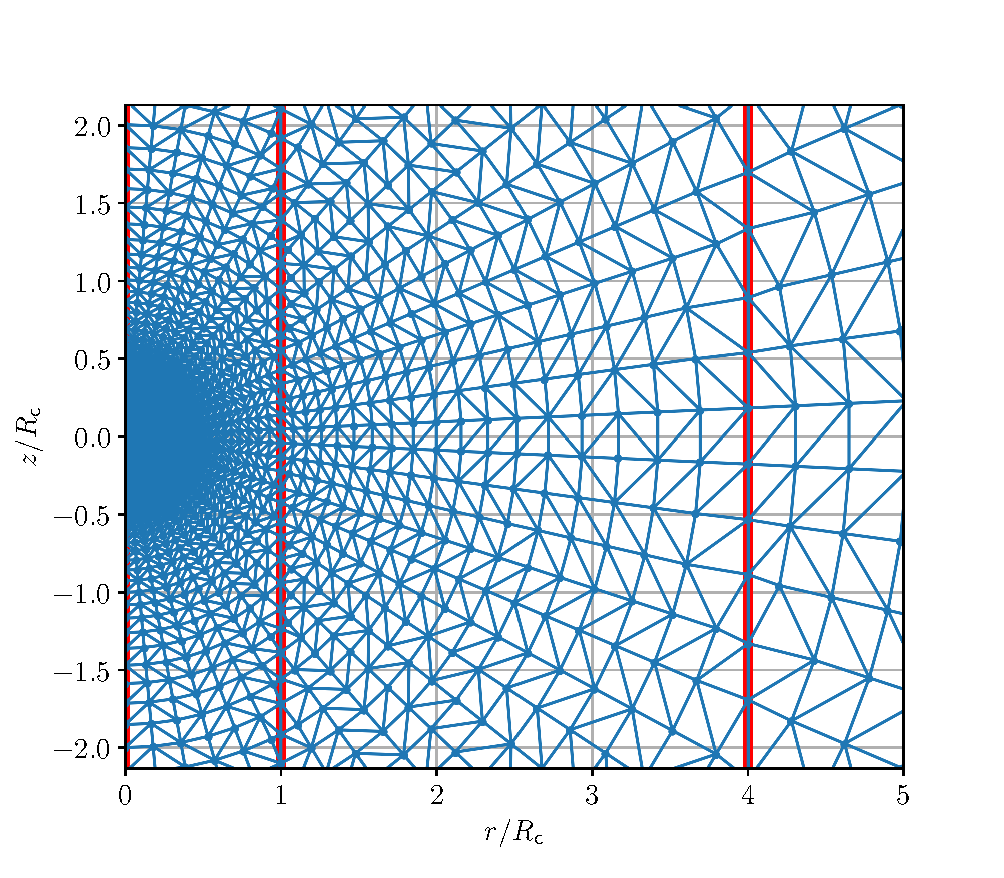
\includegraphics{plot_1_tg_2}
\caption{Триангуляция}
\label{fig:mesh_1_2}
%\label{fig:plot}
\end{figure}

\begin{figure}[H]
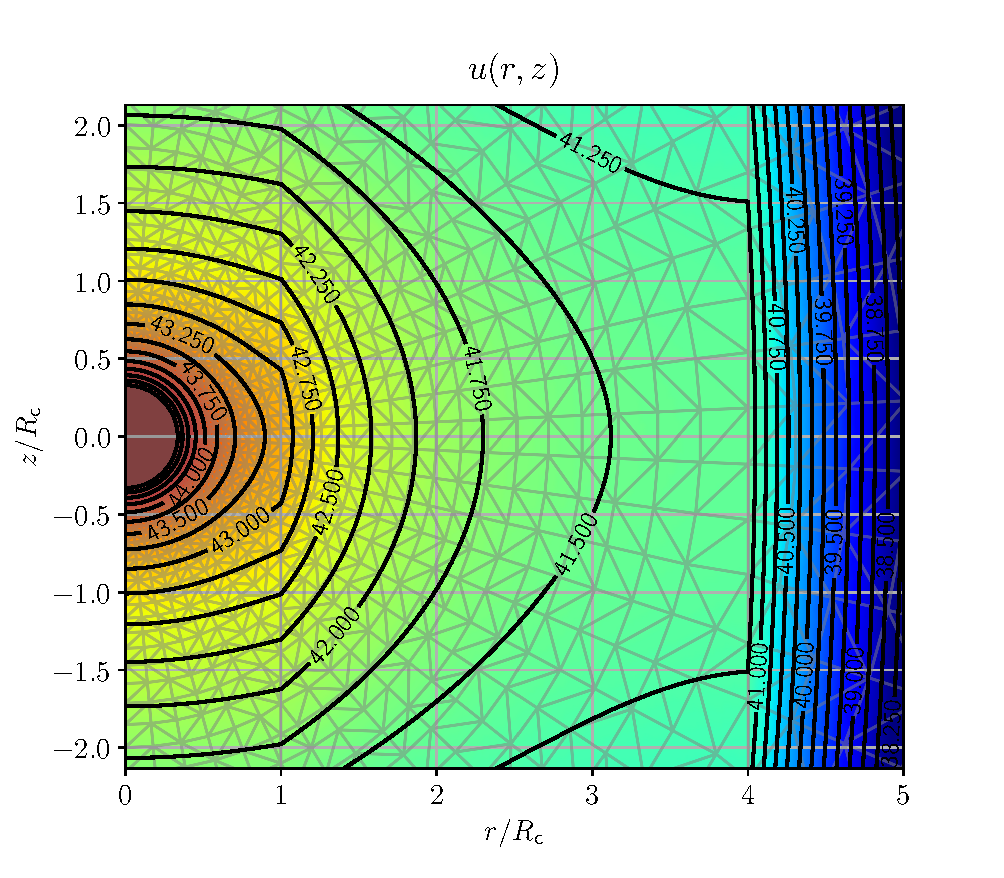
\includegraphics{plot_1_field_2}
\caption{Потенциальное поле}
\label{fig:field_1_2}
%\label{fig:plot}
\end{figure}

\begin{figure}[H]
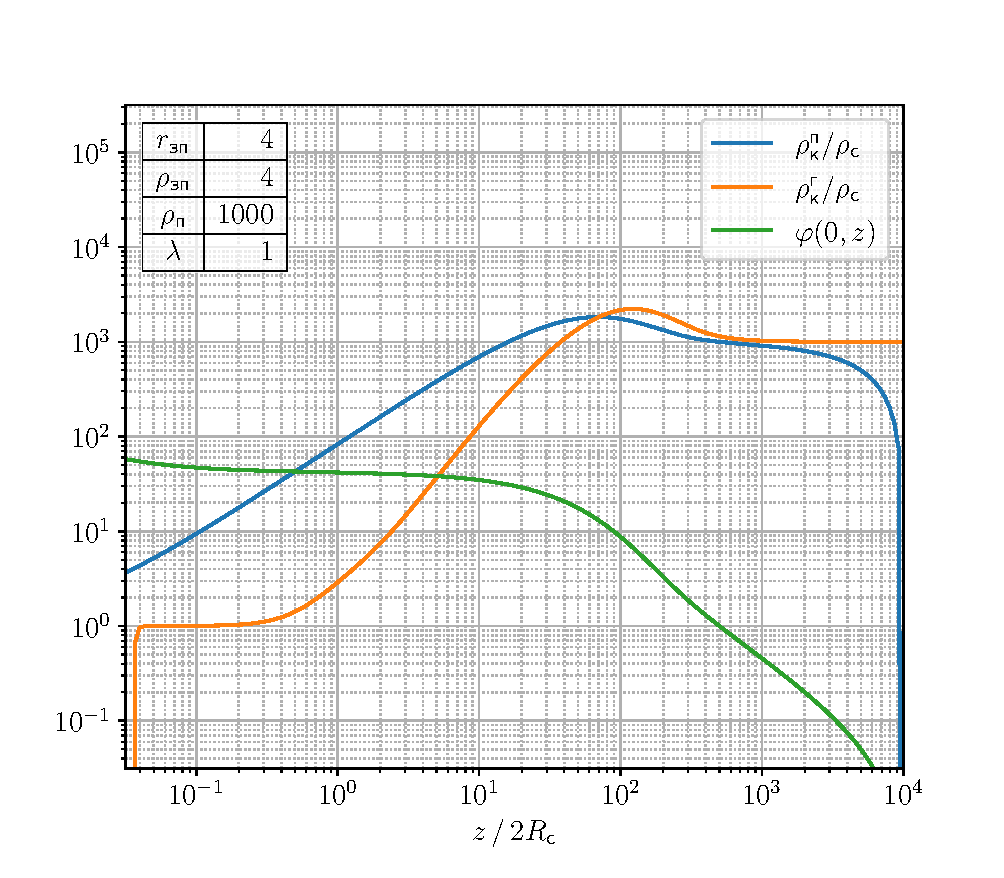
\includegraphics{plot_1_curves}
\caption{График кривых величин в скважине}
\label{fig:curves_1}
\end{figure}


\begin{figure}[H]
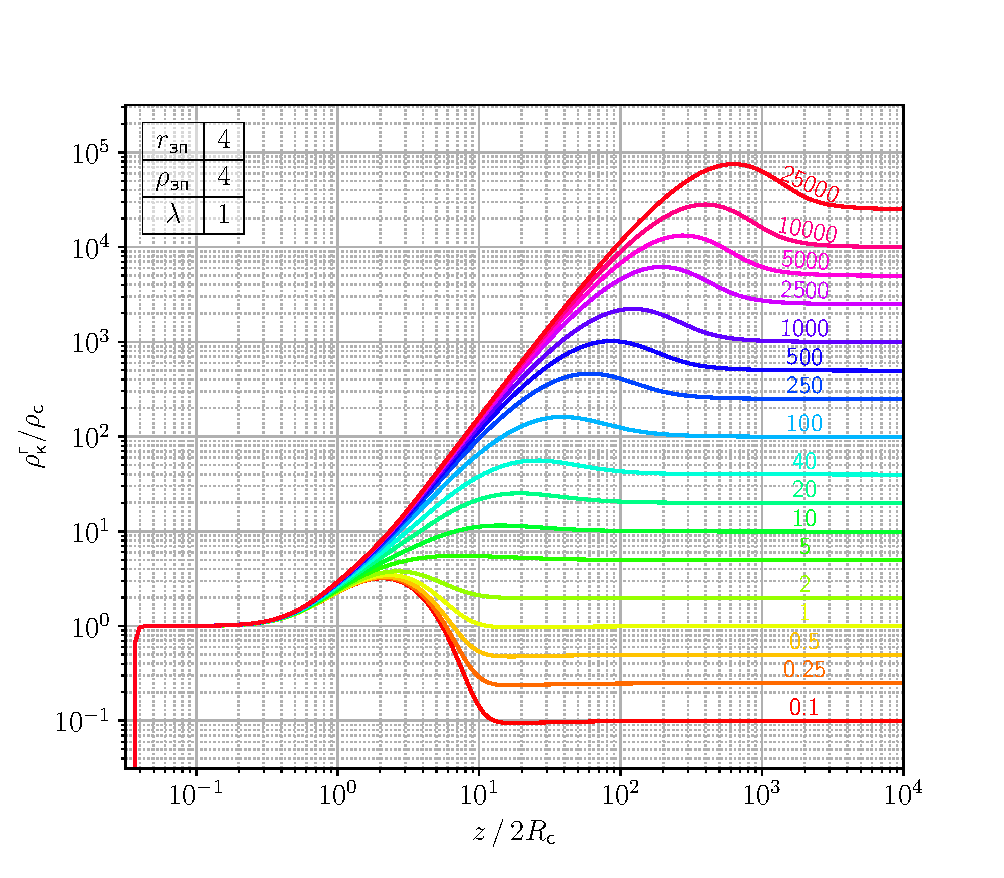
\includegraphics{plot_1_palette}
\caption{Палетка кривых}
\label{fig:palette_1}
\end{figure}

\begin{figure}[H]
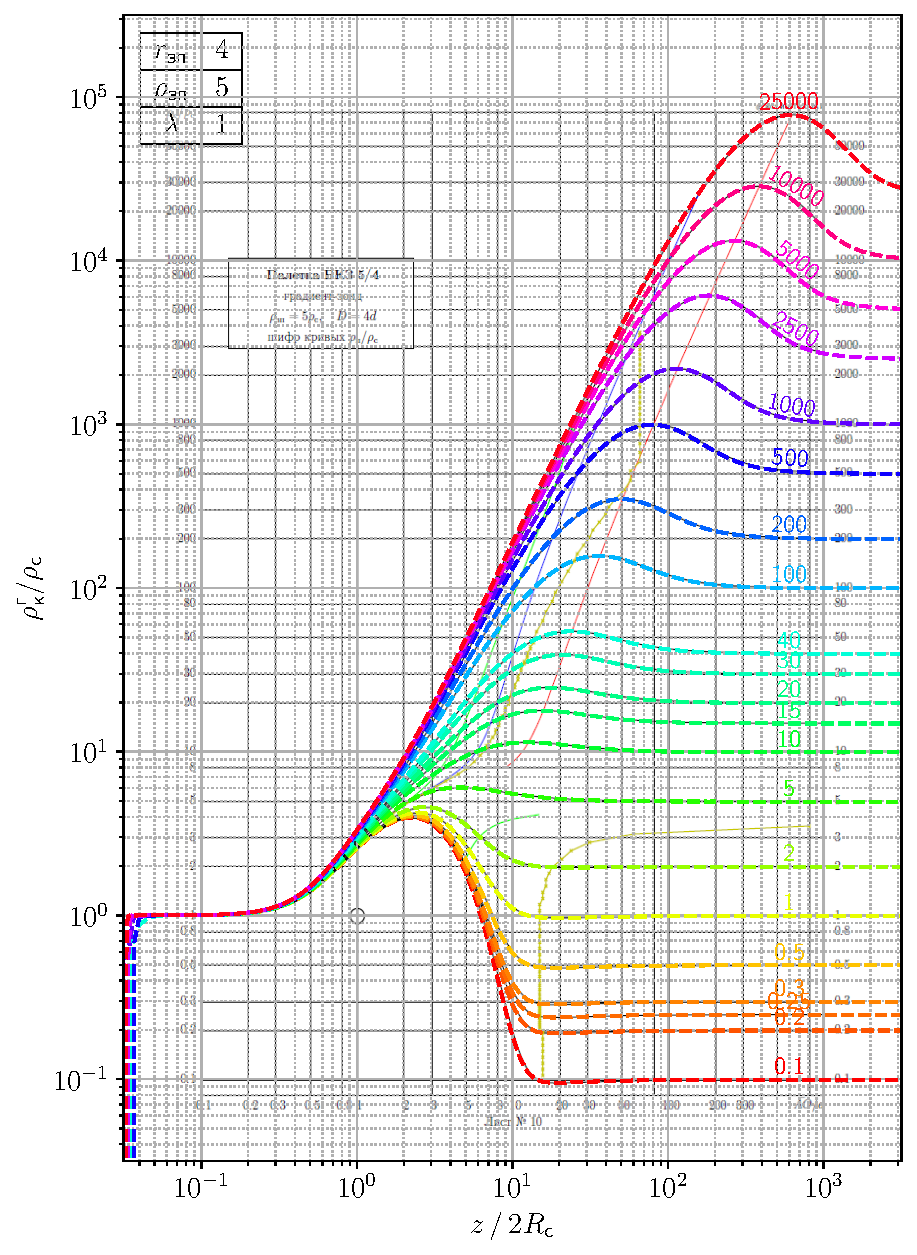
\includegraphics{plot_1_compare}
\caption{Сравнение палетки кривых}
\label{fig:compare_1}
\end{figure}


\newpage
\subsection{Модель 2}

Четырехслойная осесимметричная модель с анизотропией:

\begin{table}[h]
{\setlength\tabcolsep{2pt} \setlength\intextsep{0mm}
\begin{tabularx}{\linewidth}{r c X}
    первый слой &---& скважина (${0 < r < 1}$)
        с УЭС ${\rho_\text с = 1}$
        с коэффициентом анизотропии ${\lambda_\text{с} = 1}$, \\
    второй слой &---& промытая зона (${1 < r < r_\text{пз} = 2.2}$)
        с УЭС ${\rho_\text{пз} = 4}$
        с коэффициентом анизотропии $\lambda_\text{пз} = \lambda = 1.1$, \\
    третий слой &---& зона проникновения (${r_\text{пз} < r < r_\text{зп} = 5.8}$)
        с УЭС линейная функция от $r$ со значениями ${\rho_\text{зп}(r_\text{пз}) = \rho_\text{пз}}$
        и ${\rho_\text{зп}(r_\text{зп}) = \rho_\text{п}}$
        с коэффициентом анизотропии $\lambda_\text{зп} = \lambda = 1.1$, \\
    четвертый слой &---& пласт (${r > r_\text{зп}}$)
        с УЭС $\rho_\text{п}$
        с коэффициентом анизотропии $\lambda_\text{п} = \lambda = 1.1$.
\end{tabularx}}
\end{table}

На рис. \ref{fig:curves_2} решение потенциального поля, кажущихся сопротивлений потециал- и градиент-зондов в скважине. Решение потенциального поля на рис. \ref{fig:field_2_1} и \ref{fig:field_2_2}.

На рис. \ref{fig:field_2_2} наблюдаются разрывы градиента потенциального поля на границах зон и сингулярность поля в точке источника потенциала, означает, что это не классичекое решение задачи, а более общее --- обобщенное решение задачи. 

Время вычисления решения ${1.23 \text{ c } \pm 16.3 \text{ мс }}$, 7 проходов c 6613 узлами расчетной сетки на рис. \ref{fig:mesh_2_1} и \ref{fig:mesh_2_2}.

Решение палетки на рис. \ref{fig:palette_2} с расчетной сеткой на рис. \ref{fig:mesh_2_1}.

На рис. \ref{fig:palette_2} наблюдаются вырождение кривых в одну кривую при меньших длин зонда и асимптотическое поведение кривых при меньших длин зонда и при больших длин зонда. Асимптота при меньших длин зонда есть горизонтальная прямая со значением УЭС скважины $\rho_\text{с}$. Асимптота при больших длин зонда есть горизонтальная прямая со значением УЭС пласта $\rho_\text{п}$. Отклонение от асимптоты при больших длин зонда вызвано неким подобием краевого эффекта, возникающем при значениях коэффицинта анизотропии $\lambda \neq 1$.

Время вычисления расчетной палетки ${16.5 \text{ c } \pm 176 \text{ мс}}$, 7 проходов.

\begin{figure}[H]
\centering
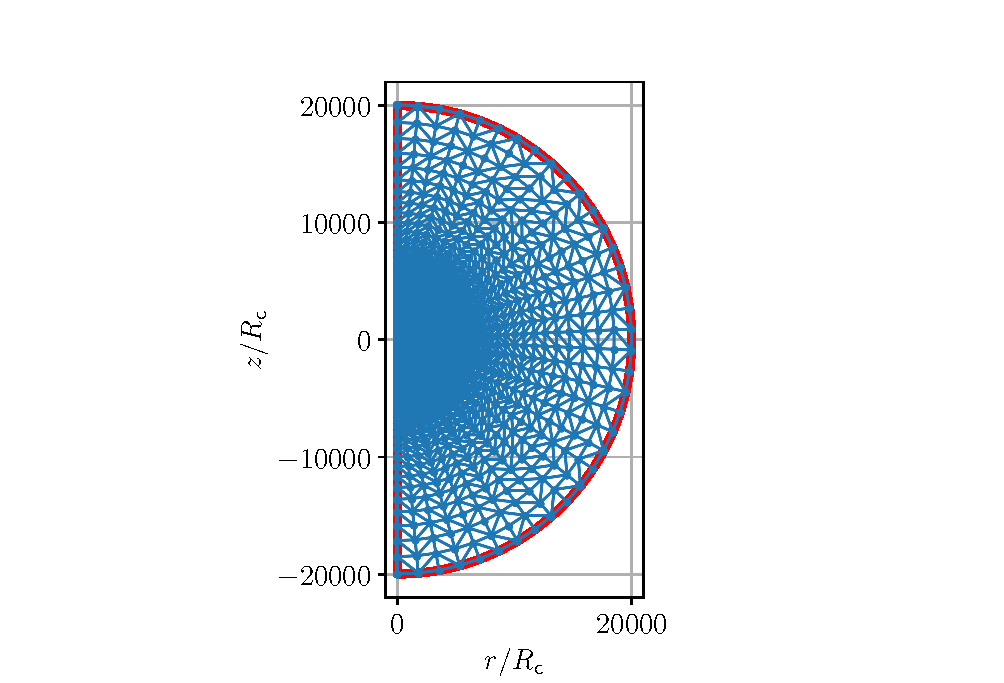
\includegraphics{plot_2_tg_1}
\caption{Триангуляция}
\label{fig:mesh_2_1}
%\label{fig:plot}
\end{figure}

\begin{figure}[H]
\centering
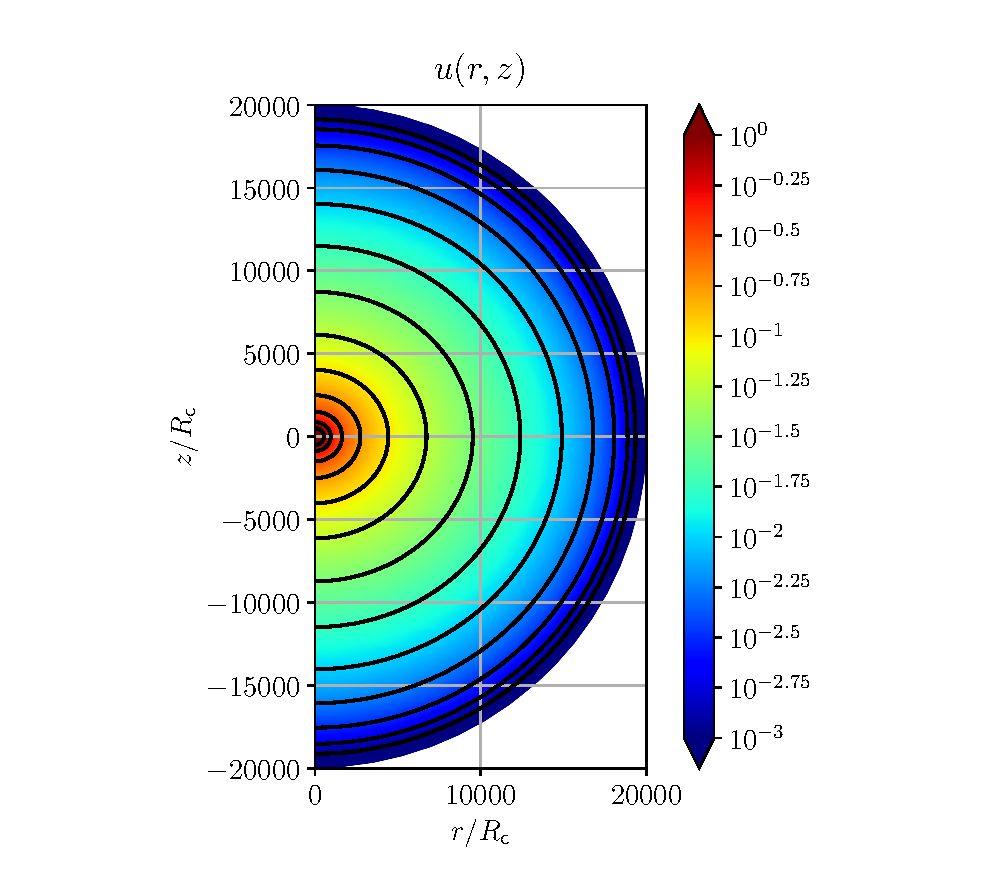
\includegraphics{plot_2_field_1}
\caption{Потенциальное поле}
\label{fig:field_2_1}
%\label{fig:plot}
\end{figure}

\begin{figure}[H]
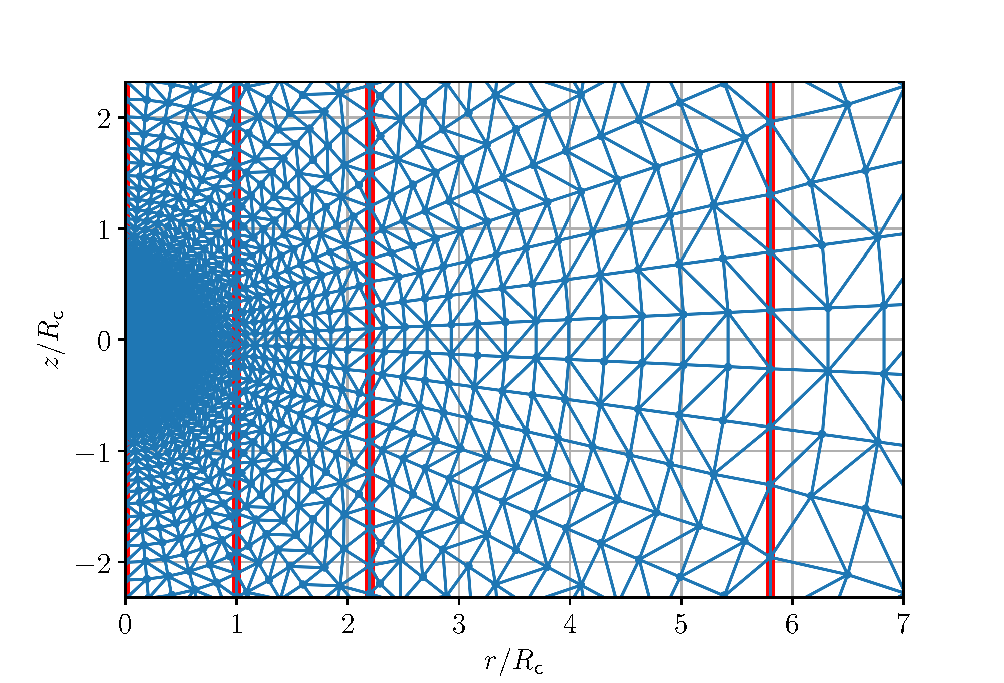
\includegraphics{plot_2_tg_2}
\caption{Триангуляция}
\label{fig:mesh_2_2}
%\label{fig:plot}
\end{figure}

\begin{figure}[H]
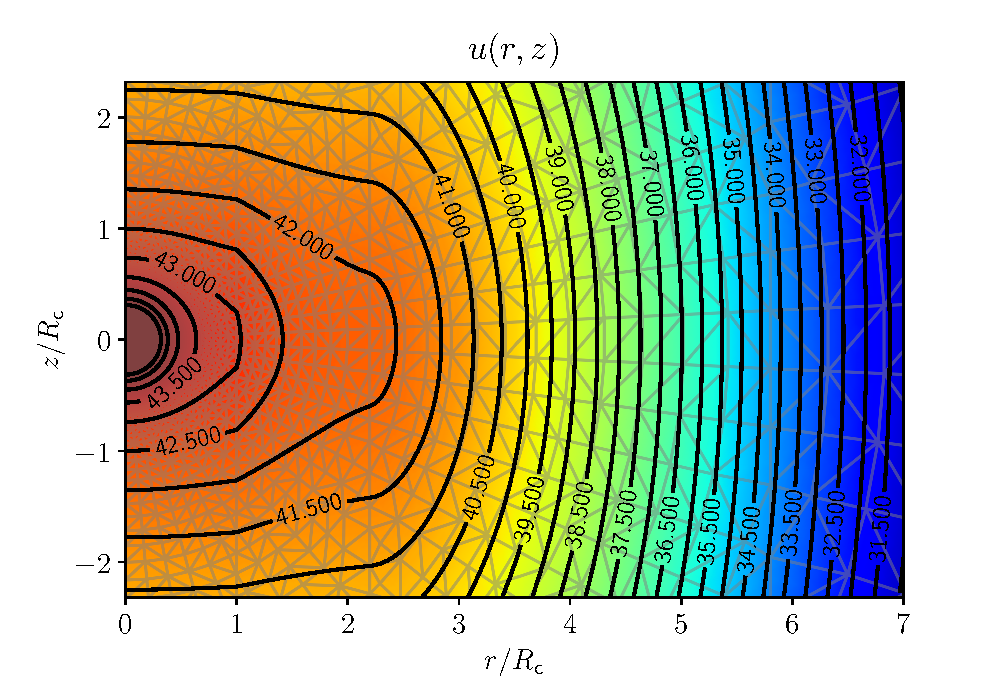
\includegraphics{plot_2_field_2}
\caption{Потенциальное поле}
\label{fig:field_2_2}
\end{figure}

\begin{figure}[H]
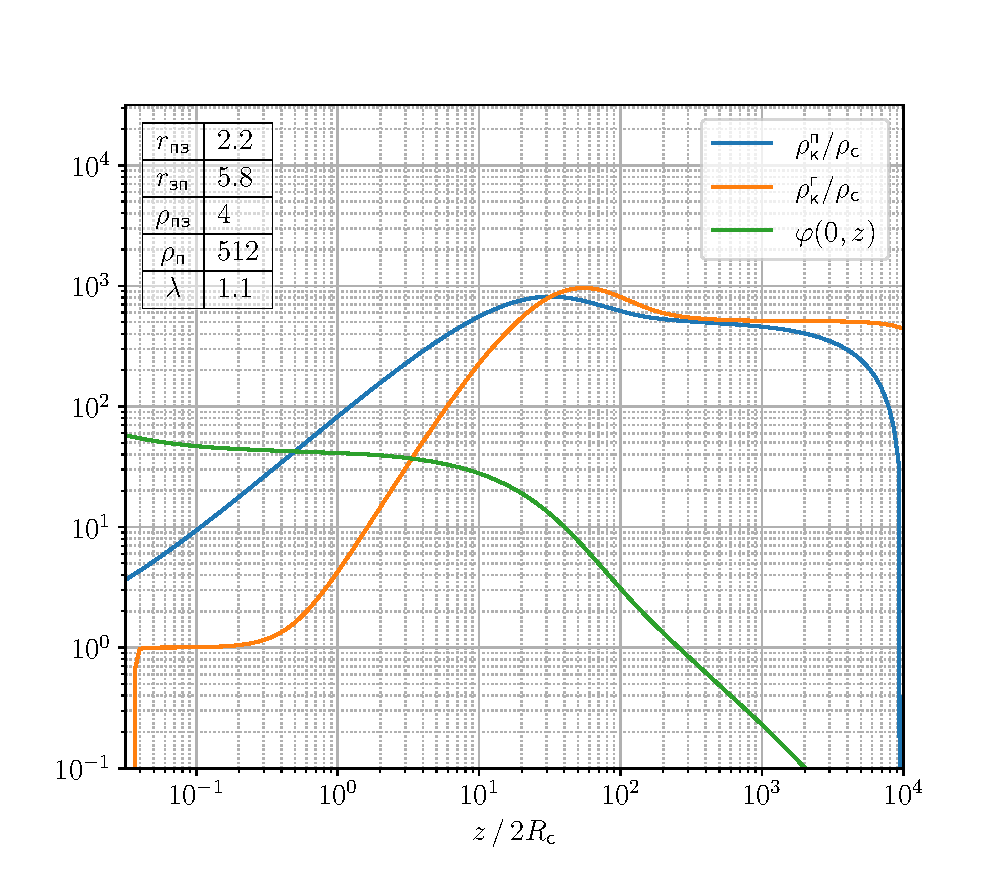
\includegraphics{plot_2_curves}
\caption{График кривых величин в скважине}
\label{fig:curves_2}
%\label{fig:plot}
\end{figure}

\begin{figure}[H]
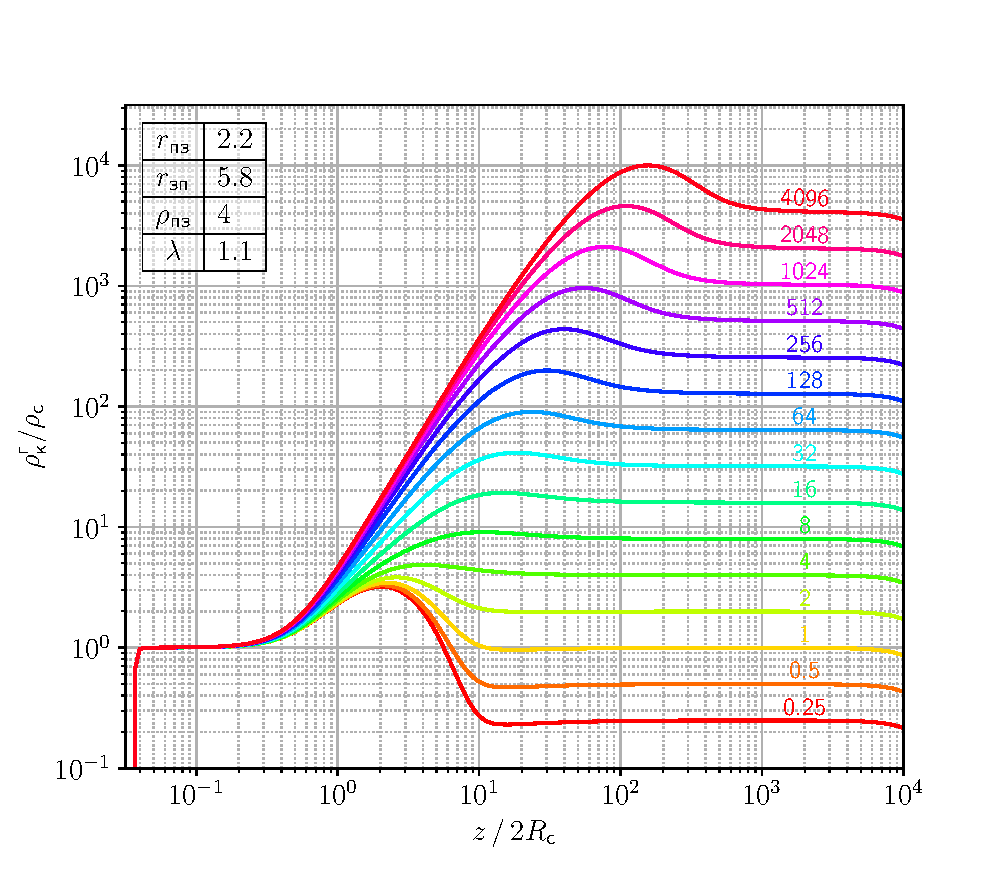
\includegraphics{plot_2_palette}
\caption{Палетка кривых}
\label{fig:palette_2}
\end{figure}

\begin{figure}[H]
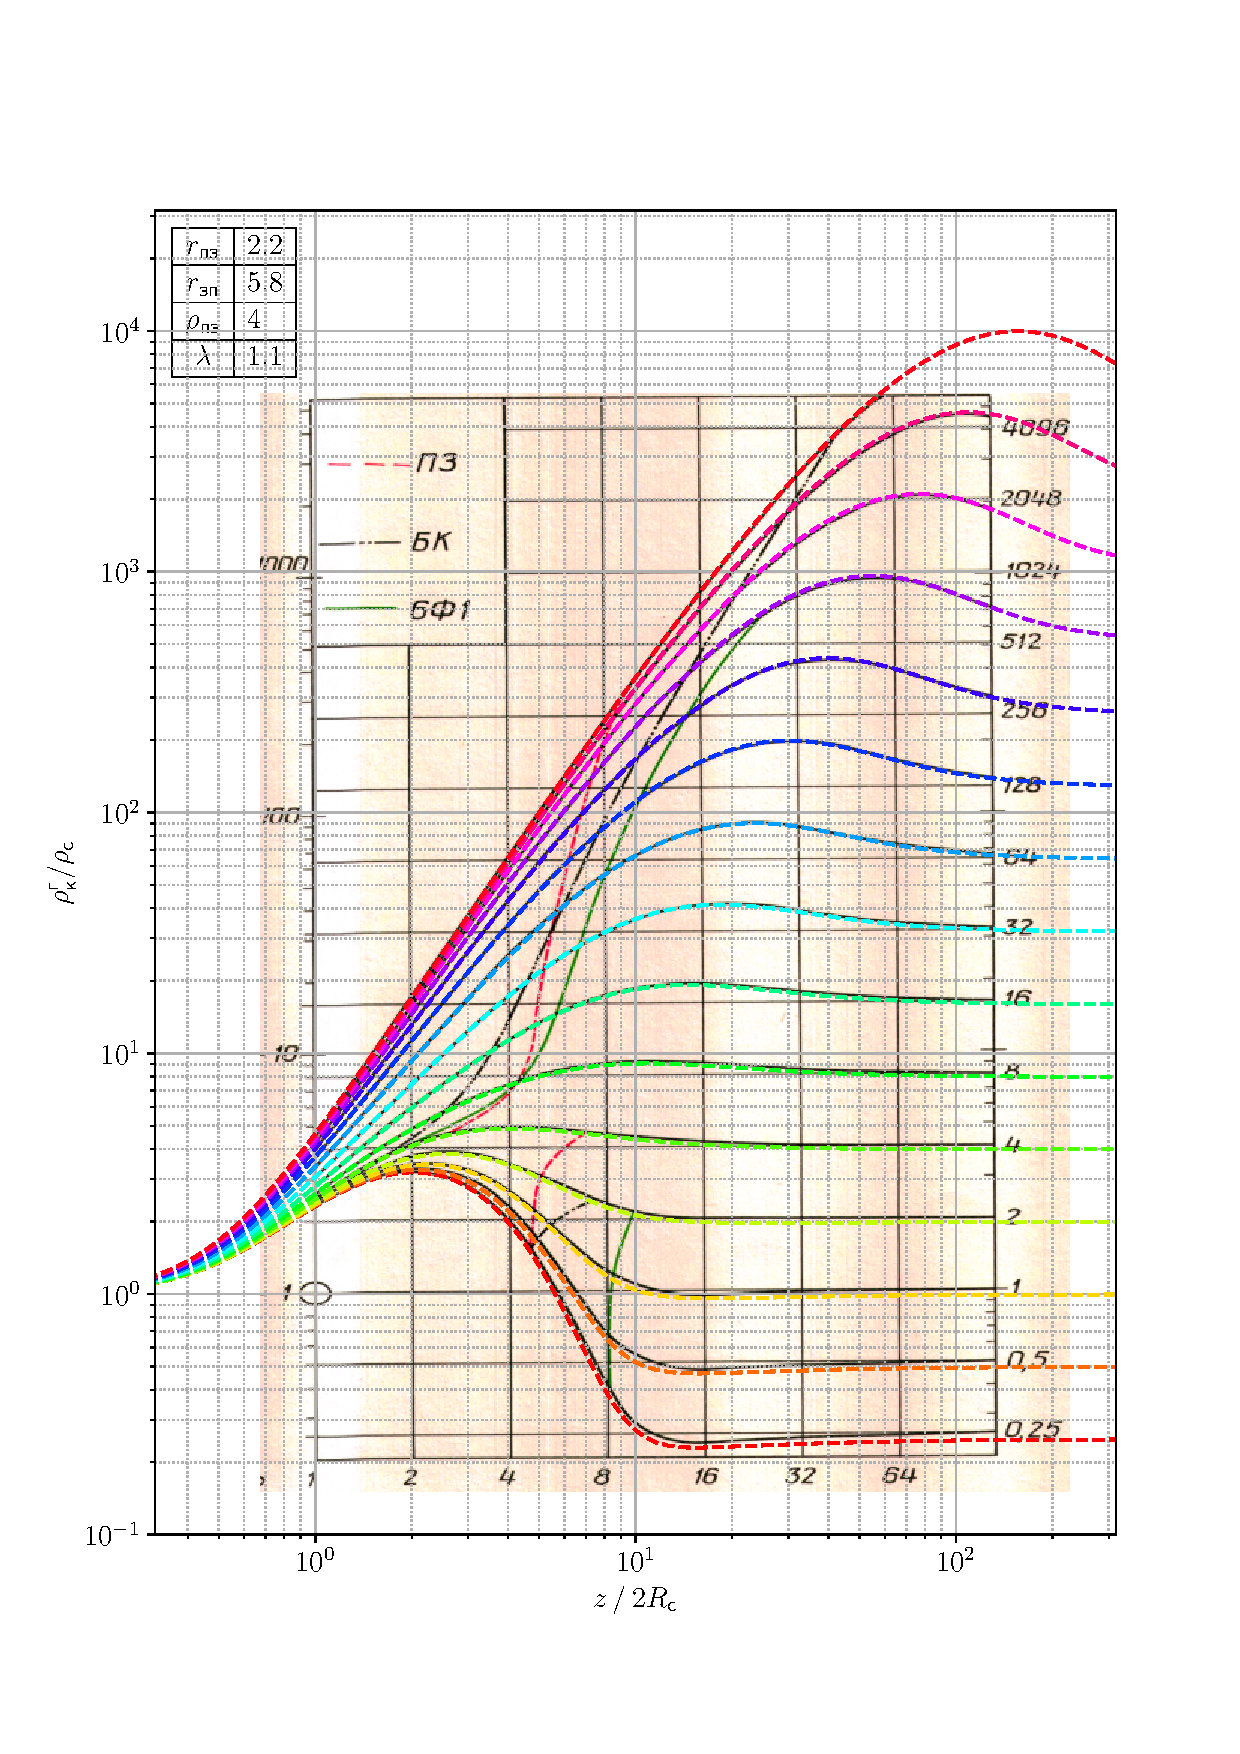
\includegraphics{plot_2_compare}
\caption{Сравнение палетки кривых}
\label{fig:compare_2}
\end{figure}

Сравнены расчетная и известная палетки на рис. \ref{fig:compare_2}. Наблюдается совпадение, означает, что способ решения верный и точный.

\clearpage
